\documentclass[
11pt, % The default document font size, options: 10pt, 11pt, 12pt
%oneside, % Two side (alternating margins) for binding by default, uncomment to switch to one side
english, % ngerman for German
singlespacing, % Single line spacing, alternatives: onehalfspacing or doublespacing
%draft, % Uncomment to enable draft mode (no pictures, no links, overfull hboxes indicated)
%nolistspacing, % If the document is onehalfspacing or doublespacing, uncomment this to set spacing in lists to single
%liststotoc, % Uncomment to add the list of figures/tables/etc to the table of contents
%toctotoc, % Uncomment to add the main table of contents to the table of contents
%parskip, % Uncomment to add space between paragraphs
%nohyperref, % Uncomment to not load the hyperref package
headsepline, % Uncomment to get a line under the header
%chapterinoneline, % Uncomment to place the chapter title next to the number on one line
%consistentlayout, % Uncomment to change the layout of the declaration, abstract and acknowledgements pages to match the default layout
]{StyleSheet} % The class file specifying the document structure

\usepackage[utf8]{inputenc} % Required for inputting international characters
\usepackage[T1]{fontenc} % Output font encoding for international characters
\usepackage{palatino} % Use the Palatino font by default
\usepackage[backend=bibtex,style=authoryear,natbib=true]{biblatex} % Use the bibtex backend with the authoryear citation style (which resembles APA)
% Refer Bibliography Resource
\usepackage[autostyle=true]{csquotes} % Required to generate language-dependent quotes in the bibliography
\usepackage[figuresleft]{rotating}

\addbibresource{example.bib} % The filename of the bibliography

\newcommand{\drawing}[2]{
\begin{sidewaysfigure}
    \centering
    \includegraphics[width=0.85\textwidth]{#1}
    \caption{#2}
\end{sidewaysfigure}
\clearpage
}

\newcommand{\drawingTwo}[2]{
\begin{sidewaysfigure}
    \centering
    \includegraphics[width=0.75\textwidth]{#1}
    \caption{#2}
\end{sidewaysfigure}
\clearpage
}

\geometry{
	paper=letterpaper, % Change to letterpaper for US letter
	inner=2.5cm, % Inner margin
	outer=3.8cm, % Outer margin
	bindingoffset=.5cm, % Binding offset
	top=1.5cm, % Top margin
	bottom=1.5cm, % Bottom margin
	%showframe, % Uncomment to show how the type block is set on the page
}

\thesistitle{GT Pioneer} 
% Your thesis title, this is used in the title and abstract, print it elsewhere with \ttitle

\supervisor{Dr. Raghuram \textsc{Pucha}} 
% Your supervisor's name, this is used in the title page, print it elsewhere with \supname

\examiner{} 
% Your examiner's name, this is not currently used anywhere in the template, print it elsewhere with \examname

\degree{ME1770} 
% Your degree name, this is used in the title page and abstract, print it elsewhere with \degreename

\author{Vishakh \textsc{Kumar}} 
% Your name, this is used in the title page and abstract, print it elsewhere with \authorname

\addresses{} 
% Your address, this is not currently used anywhere in the template, print it elsewhere with \addressname

\subject{ME 1770} 
% Your subject area, this is not currently used anywhere in the template, print it elsewhere with \subjectname

\keywords{Georgia Tech, Mars Rover, Pioneer} 
% Keywords for your thesis, this is not currently used anywhere in the template, print it elsewhere with \keywordnames

\university{\href{http://www.gatech.edu}{Georgia Institute of Technology}}

\department{\href{http://me.gatech.edu}{George W Woodruff School of Mechanical Engineering}}
% Your department's name and URL, this is used in the title page and abstract, print it elsewhere with \deptname

\group{\href{https://github.com/vishakhkumar/ME1770}{Group X}}

\faculty{\href{http://faculty.university.com}{Faculty Name}}
% Your faculty's name and URL, this is used in the title page and abstract, print it elsewhere with \facname

\AtBeginDocument{
\hypersetup{pdftitle=\ttitle} % Set the PDF's title to your title
\hypersetup{pdfauthor=\authorname} % Set the PDF's author to your name
\hypersetup{pdfkeywords=\keywordnames} % Set the PDF's keywords to your keywords
}

\begin{document}

\frontmatter % Use roman page numbering style (i, ii, iii, iv...) for the pre-content pages
\pagestyle{plain} % Default to the plain heading style until the thesis style is called for the body content

\begin{titlepage}
\begin{center}

\vspace*{.06\textheight}
{\scshape\LARGE \univname\par}\vspace{1.5cm} % University name
\textsc{\Large Project Report}\\[0.5cm] % Thesis type

\HRule \\[0.4cm] % Horizontal line
{\huge \bfseries \ttitle\par}\vspace{0.4cm} % Thesis title
\HRule \\[1.5cm] % Horizontal line

\begin{minipage}[t]{0.4\textwidth}
\begin{flushleft} \large
\emph{Author:}\\
\href{http://www.johnsmith.com}{\authorname} % Author name - remove the \href bracket to remove the link
\end{flushleft}
\end{minipage}
\begin{minipage}[t]{0.4\textwidth}
\begin{flushright} \large
\emph{Instructor:} \\
\href{http://www.me.gatech.edu/faculty/pucha}{\supname} % Supervisor name - remove the \href bracket to remove the link  
\end{flushright}
\end{minipage}\\[3cm]

\vfill

\large \textit{A report submitted in fulfillment of the requirements\\ for the team project of ME 1770}\\[0.3cm] % University requirement text
\textit{in the}\\[0.4cm]
\groupname\\\deptname\\[2cm] % Research group name and department name

\vfill

{\large \today}\\[4cm] % Date
%\includegraphics{Logo} % University/department logo - uncomment to place it

\vfill
\end{center}
\end{titlepage}


\mainmatter % Begin numeric (1,2,3...) page numbering
\pagestyle{thesis} % Return the page headers back to the "thesis" style

\chapter{Project Ideation}

\section{Project Proposal}
\subsection{Description of Product / Structure: Describe the creative ideation and what is new?}

Our product is a Mars capable ATV. We began with the idea of the standard ATV, coupled with the idea of a manned Mars rover. By combining these two concepts, we were able to create a more agile vehicle capable of handling Mars’ low gravity and dusty environment. The combination of a pressurized capsule in an off-road vehicle can be challenging but the benefits would be immense in creating robust vehicles for a manned colony on Mars.

\subsection{Description of subsystem}

\begin{center}
\begin{tabular}{lll}
\hline
Subsystem & Description\\
\hline
Orbital Deployment & Circular parachute and coiled spring shocks.\\
Grabbers & Pivoting arm with ball socket and grabbing hands.\\
Suspension & Coil spring shocks, double A-frame suspension and tire rods.\\
Chassis & Triangular truss support frame. \\
Tires & Cylindrical tires with embossed treads. \\
Controls & Joystick,Displays, Plexiglas encased w/ rectangular control panel.\\
Cockpit & Oblong shaped cockpit \\
Powertrain & Circular Motor with chain drive to rear axle with rear diff.\\
Charging & Rectangular solar cells on roof. \\
Science/Storage & Large prismed storage area in back of ATV. \\
Communication System & Conic Satellite Dish. \\
Lighting & Semi-Paraboloid lights mounted on front of ATV. \\
\hline
\end{tabular}
\end{center}

\subsection{Subassembly Functionality}
\begin{center}
\begin{tabular}{lll}
\hline
Subsystem & Functionality\\
\hline
Orbital Deployment & Landing Gear when ATV is dropped from orbit. \\
Grabbers & Grabs materials for data inspection.\\
Suspension & Absorbs shocks from planetary terrain. \\
Chassis & Beefy frame for surviving rough conditions.\\
Tires & Extreme grip to handle unexpected terrain. \\
Controls & Steering, cockpit, seating, etc.\\
Cockpit & Location of Controls\\
Powertrain & Electric drivetrain, differential. \\
Charging & Solar cells from roof to charge batteries behind cockpit. \\
Science/Storage & Large storage area in back of ATV to collect data/samples. \\
Communication System & Antenna to communicate with base. \\
Lighting & To maintain visibility once night falls or in sandstorms.\\
\hline
\end{tabular}
\end{center}

\subsection{Allocation for each member}

\begin{center}
\begin{tabular}{lll}
\hline
Subsystem & Member& Complexity\\
\hline
Orbital Deployment & Vishakh Kumar& Medium\\
Grabbers & Justin Sackett & Hard\\
Suspension & Asimm Hirani & Medium\\
Chassis & Juan Rodriguez & Hard\\
Tires & Auston Ferrarer& Easy\\
Controls & Vishakh Kumar & Hard\\
Cockpit & Vishakh Kumar & Easy\\
Powertrain & Asimm Hirani & Hard\\
Charging & Vishakh Kumar & Easy \\
Science/Storage & Auston Ferrarer & Medium\\
Communication System & Juan Rodriguez & Medium\\
Lighting & Justin Sackett& Easy\\
\hline
\end{tabular}
\end{center}

\subsection{Briefly explain what new functionalities (system and sub-system ) you are planning to add. How your product is different from existing products:}

This design differs from the traditional ATV because it has a improved suspension system for travel along Martian terrain. The ATV will be able to withstand orbital entry into the Martian landscape through its improved suspension and parachute for controlled descent. Additionally for increased driver visibility the pressurized cabin is built with GT-Superglass® which has the material strength of hardened steel and the weight of titanium. With this glass our vehicle will be able to withstand sandstorms containing heavy debris.

\subsection{Picture of  the Proposed System (or Similar System): (please include a reference if you are using pictures from internet). You can also include conceptual sketch.}
\begin{center}
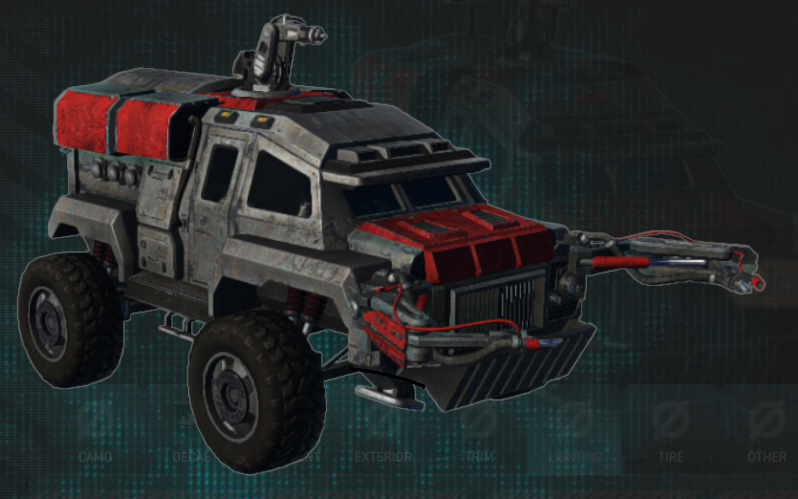
\includegraphics[width=0.75\textwidth]{a-1-1-ProjectIdeation/b-1-ProjectProposal/c-1-Images/Planetside.png} \\
(Daybreak Games: Planetside 2 ANT Vehicle Concept)

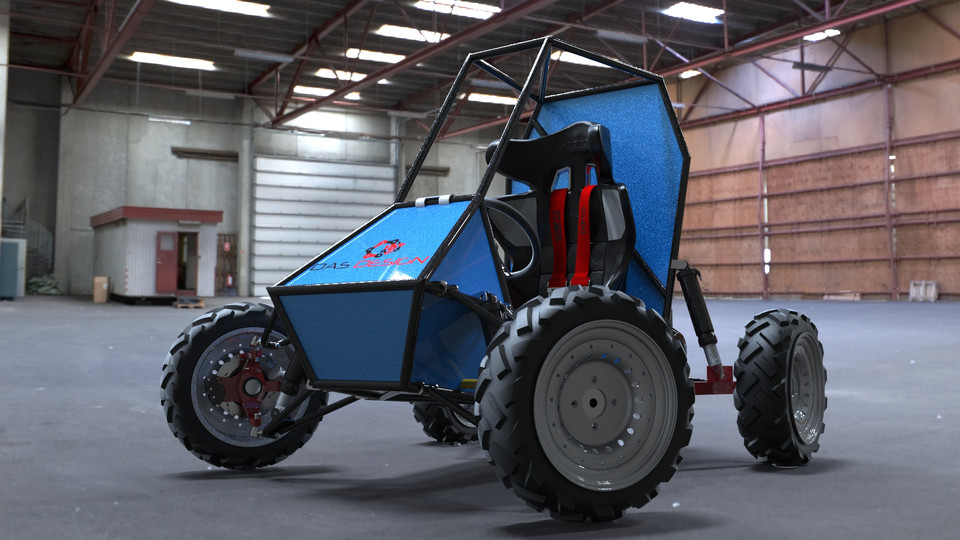
\includegraphics[width=0.75\textwidth]{a-1-1-ProjectIdeation/b-1-ProjectProposal/c-1-Images/BAJA.jpeg} \\
(https://grabcad.com/library/baja-atv-1 - BAJA SAE India Team)
\end{center}


\clearpage
 \section{Project Management}
 

Insert spiel about ProjectManagement.

\subsection{PartDistribution}
\subsubsection{Allocating subsystems among team members}

An important element of team success lies in allocating tasks to team members equitably. We kept in mind two factors while allocating tasks:

  - the set of tasks that has to be completed (which may be one task or it may be several) and
  - the set of individuals (the team members) able to complete them.

Given each team member's skill level and complexity of the part, we assigned tasks as shown in the Project Proposal (I forgot the table number).

Further description

Since the cockpit and the controls were interrelated task, it was decided to allocate both tasks to the same person.

This probably should be filled out more.


\subsection{Planning}
Insert spiel about planning.


\subsection{Timeline}
Planning our project was simple using Gantt chart created in an Excel sheet. We opted to finish our tasks earlier than suggested by the Gantt chart provided to us by our instructor due to our experience with Solidworks and inreased workload at the end of the semester from other subjects. 
We've included an image of our Gantt chart in the figure \ref{fig:GanttChart} on page \pageref{fig:GanttChart}.\\
 A detailed view of our timeline can be found at \url{https://github.com/vishakhkumar/ME1770}

\begin{figure}[!ht]
\centering
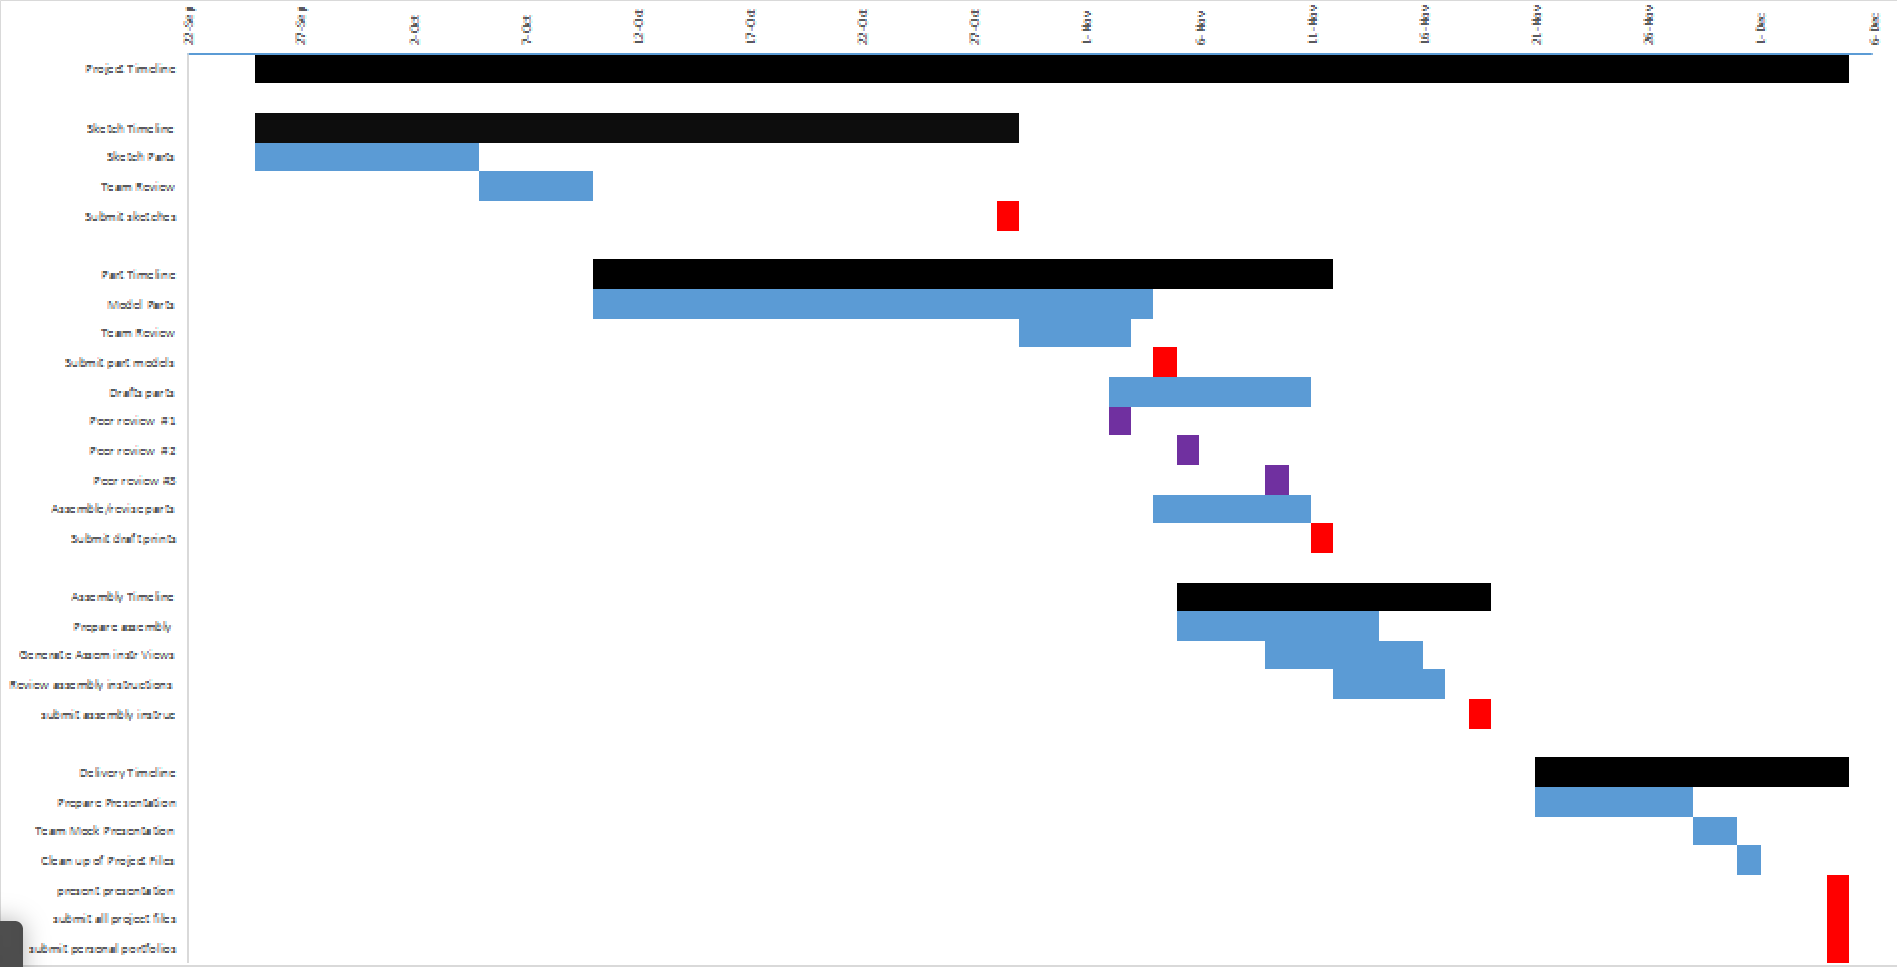
\includegraphics[angle=90,height=\textheight]{a-1-1-ProjectIdeation/b-2-ProjectManagement/Timeline.png}
\caption{Gantt Chart}
\label{fig:GanttChart}
\end{figure}





\chapter{Preliminary Design}

Insert spiel about PreliminaryDesign.

\section{Conceptual Sketches}
Our project was fairly ambitious in that we combined two very different worlds - the rough and tumble world of off-road vehicles and the pressurized environments of space vehicles. Conceptual drawings were invaluable in sketching out a basic idea of what this vehicle would look like.

\drawing{/a-1-2-PreliminaryDesign/b-3-Multiview/Asimm/IMG_1811.JPG}{Hirani, Asimm: Gear One}
\drawing{/a-1-2-PreliminaryDesign/b-3-Multiview/Asimm/IMG_1812.JPG}{Hirani, Asimm: Disc BRake}
\drawing{/a-1-2-PreliminaryDesign/b-3-Multiview/Asimm/IMG_1813.JPG}{Hirani, Asimm: Upright}
\drawing{/a-1-2-PreliminaryDesign/b-3-Multiview/Asimm/IMG_1814.JPG}{Hirani, Asimm: Motor}
 
\clearpage

\drawing{/a-1-2-PreliminaryDesign/b-3-Multiview/Auston/3DPrinter.jpg}{Ferrarer, Auston: 3D Printer}
\drawing{/a-1-2-PreliminaryDesign/b-3-Multiview/Auston/Bed.jpg}{Ferrarer, Auston: Bed}
\drawing{/a-1-2-PreliminaryDesign/b-3-Multiview/Auston/Helmet.jpg}{Ferrarer, Auston: Helmet}
\drawing{/a-1-2-PreliminaryDesign/b-3-Multiview/Auston/RearHatch.jpg}{Ferrarer, Auston: Rear Hatch}
 
\clearpage

\drawing{/a-1-2-PreliminaryDesign/b-2-Isometric/Juan}{Rodriguez, Juan: }
 
\clearpage

\drawing{/a-1-2-PreliminaryDesign/b-3-Multiview/Justin}{Sackett, Justin: }


\drawing{/a-1-2-PreliminaryDesign/b-3-Multiview/Justin/IMG_1554.JPG}{Sackett, Justin: }
\drawing{/a-1-2-PreliminaryDesign/b-3-Multiview/Justin/IMG_1555.JPG}{Sackett, Justin: }
\drawing{/a-1-2-PreliminaryDesign/b-3-Multiview/Justin/IMG_1556.JPG}{Sackett, Justin: }
\drawing{/a-1-2-PreliminaryDesign/b-3-Multiview/Justin/IMG_1557.JPG}{Sackett, Justin: }
\drawing{/a-1-2-PreliminaryDesign/b-3-Multiview/Justin/IMG_1558.JPG}{Sackett, Justin: }
\drawing{/a-1-2-PreliminaryDesign/b-3-Multiview/Justin/IMG_1559.JPG}{Sackett, Justin: }
\drawing{/a-1-2-PreliminaryDesign/b-3-Multiview/Justin/IMG_1560.JPG}{Sackett, Justin: }
 
\clearpage

\drawingThree{/a-1-2-PreliminaryDesign/b-1-Conceptual/Vishakh}{Kumar, Vishakh: }

\clearpage


\section{Isometric Sketches}
After sketching out our conceptual drawings and allocating tasks between team members, we then proceded to create isometric drawings of each assembly and the top level subassemblies.
This helped us refine our ideas about what our parts would look like and how we could improve them.
As our product was fairly complicated, we also had the benefit of improving our drawing skills - more than a few parts had interesting features that were a challenge to draw.

\subsection{Assim}
% \drawing{/a-1-2-PreliminaryDesign/b-1-Conceptual/Assim}{Hirani, Asimm: }
\drawing{/a-1-2-PreliminaryDesign/b-1-Conceptual/Assim/IMG_1809}{Hirani, Asimm: Suspension}
\drawing{/a-1-2-PreliminaryDesign/b-1-Conceptual/Assim/IMG_1810}{Hirani, Asimm: Powertrain}
\drawing{/a-1-2-PreliminaryDesign/b-1-Conceptual/Assim/IMG_1815}{Hirani, Asimm: Scientiic Storage}


\subsection{ Auston}
\drawing{/a-1-2-PreliminaryDesign/b-3-Multiview/Auston/3DPrinter.jpg}{Ferrarer, Auston: 3D Printer}
\drawing{/a-1-2-PreliminaryDesign/b-3-Multiview/Auston/Bed.jpg}{Ferrarer, Auston: Bed}
\drawing{/a-1-2-PreliminaryDesign/b-3-Multiview/Auston/Helmet.jpg}{Ferrarer, Auston: Helmet}
\drawing{/a-1-2-PreliminaryDesign/b-3-Multiview/Auston/RearHatch.jpg}{Ferrarer, Auston: Rear Hatch}


\subsection{Juan}
\drawing{/a-1-2-PreliminaryDesign/b-2-Isometric/Juan}{Rodriguez, Juan: }


\subsection{Justin}
\drawing{/a-1-2-PreliminaryDesign/b-3-Multiview/Justin}{Sackett, Justin: }


\drawing{/a-1-2-PreliminaryDesign/b-3-Multiview/Justin/IMG_1554.JPG}{Sackett, Justin: }
\drawing{/a-1-2-PreliminaryDesign/b-3-Multiview/Justin/IMG_1555.JPG}{Sackett, Justin: }
\drawing{/a-1-2-PreliminaryDesign/b-3-Multiview/Justin/IMG_1556.JPG}{Sackett, Justin: }
\drawing{/a-1-2-PreliminaryDesign/b-3-Multiview/Justin/IMG_1557.JPG}{Sackett, Justin: }
\drawing{/a-1-2-PreliminaryDesign/b-3-Multiview/Justin/IMG_1558.JPG}{Sackett, Justin: }
\drawing{/a-1-2-PreliminaryDesign/b-3-Multiview/Justin/IMG_1559.JPG}{Sackett, Justin: }
\drawing{/a-1-2-PreliminaryDesign/b-3-Multiview/Justin/IMG_1560.JPG}{Sackett, Justin: }


\subsection{Vishakh}
\drawingThree{/a-1-2-PreliminaryDesign/b-1-Conceptual/Vishakh}{Kumar, Vishakh: }



\section{Multiview Sketches}


\newcommand{\Multiview}[1]{
 \subsection{#1}
 \input{a-1-2-PreliminaryDesign/b-3-Multiview/#1/#1.tex} 
 \clearpage
}

\Multiview{Asimm}
\Multiview{Auston}
\Multiview{Juan}
\Multiview{Justin}
\Multiview{Vishakh}




\chapter{DetailDesign}

Insert spiel about DetailDesign.

\section{Antenna}
<<<<<<< HEAD
\drawing{a-1-4-ManufacturingWorkingDrawing/b-3-ExplodedView/c-Antenna/AntennaAssemblyExploded.JPG}{Exploded View of Antenna Assembly}
=======
\drawingTwo{a-1-4-ManufacturingWorkingDrawing/b-3-ExplodedView/c-Antenna/AntennaAssemblyExploded.JPG}{Exploded View of Antenna Assembly}
>>>>>>> b26c8c7fe51429f8ced673c0452ed2308f1da92f


\section{Cockpit}
\newcommand{\DetailDesignCockpit}[2]{\drawing{/a-1-3-DetailDesign/b-Cockpit/#1}{Kumar, Vishakh: #2}
\DetailDesignCockpit{LIGHTBASE.JPG}{Light Base}
\DetailDesignCockpit{LIGHTSCREWS.JPG}{Light Screws}
\DetailDesignCockpit{LED_Work_light_27w.JPG}{LED Work Light}


\section{Joystick}
\DetailDesignDrawing{a-1-3-DetailDesign/b-Joystick/Joystick.png}{\vishakh Joystick View 1}
\DetailDesignDrawing{a-1-3-DetailDesign/b-Joystick/Joystick1.png}{\vishakh Joystick View 2}
\DetailDesignDrawing{a-1-3-DetailDesign/b-Joystick/Joystick2.png}{\vishakh Joystick View 3}
\DetailDesignDrawing{a-1-3-DetailDesign/b-Joystick/Joystick3.png}{\vishakh Joystick View 4}


\section{MechanicalDisplay}
\WorkingDrawing{a-1-4-ManufacturingWorkingDrawing/b-1-WorkingDrawing/c-MechanicalDisplay/MechanicalDisplay.JPG}{\vishakh Mechanical Display}




\chapter{ManufacturingWorkingDrawing}
Insert spiel about ManufacturingWorkingDrawing.

\WorkingDrawing{Antenna}
\WorkingDrawing{Chassis}
\WorkingDrawing{Grabber}
\WorkingDrawing{Suspension}

\WorkingDrawing{3DPrinter}
\WorkingDrawing{Bed}
\WorkingDrawing{CabinetDoor}
\WorkingDrawing{Chassis}
\WorkingDrawing{DoorAndHinge}
\WorkingDrawing{ExteriorShell}
\WorkingDrawing{Helmet}

% \WorkingDrawing{Cockpit}
% \WorkingDrawing{Joystick}
% \WorkingDrawing{MechanicalDisplay}

\section{Working Drawings}
A product cannot be counted as finished unless there are plans to manufacture that product. While the plans for our product is definitely beyond the ability of a student run organization (or small countries), 
we've added working drawings to highlight important features and dimensions of our work.

\newcommand{\WorkingDrawing}[1]{
 \subsection{#1}
 \input{a-1-4-ManufacturingWorkingDrawing/b-1-WorkingDrawing/c-#1/#1.tex}
 }


\newcommand{\AssemblyInstructionManual}[1]{
 \subsection{#1}
 \input{a-1-4-ManufacturingWorkingDrawing/b-2-AssemblyInstructionManual/c-#1/#1.tex}
 }


\newcommand{\AssemblyManualStep}[4]{
\subsubsection{Step #1}
\begin{center}
#3
\begin{figure}[!ht]
\centering
\includegraphics[height=0.70\textheight]{#2}
\caption{#4}
\end{figure}
\end{center}
\clearpage
}

\newcommand{\AssemblyManualStepTwo}[4]{
\subsubsection{Step #1}
\begin{center}
#3
\begin{figure}[!ht]
\centering
\includegraphics[width=0.90\textwidth]{#2}
\caption{#4}
\end{figure}
\end{center}
}

\AssemblyInstructionManual{Antenna}
\clearpage
\AssemblyInstructionManual{Grabber}
\clearpage
\AssemblyInstructionManual{Lights}
\clearpage
\AssemblyInstructionManual{Suspension}
\clearpage
\AssemblyInstructionManual{3DPrinter}
\clearpage
\AssemblyInstructionManual{FlexBed}
\clearpage
\AssemblyInstructionManual{Helmet}
\clearpage
\AssemblyInstructionManual{Hinge}

% \AssemblyInstructionManual{Cockpit}
% \AssemblyInstructionManual{Joystick}
% \AssemblyInstructionManual{MechanicalDisplay}




\clearpage
\section{ExplodedView}
Insert spiel about ExplodedView.

\subsection{Antenna}
<<<<<<< HEAD
\drawing{a-1-4-ManufacturingWorkingDrawing/b-3-ExplodedView/c-Antenna/AntennaAssemblyExploded.JPG}{Exploded View of Antenna Assembly}
=======
\drawingTwo{a-1-4-ManufacturingWorkingDrawing/b-3-ExplodedView/c-Antenna/AntennaAssemblyExploded.JPG}{Exploded View of Antenna Assembly}
>>>>>>> b26c8c7fe51429f8ced673c0452ed2308f1da92f


\subsection{Lights}
\newcommand{\AssemblyManualLights}[3]{
\subsubsection{Step #1}
\begin{center}
#3
\begin{figure}[!ht]
\includegraphics[width=0.85\textwidth]{/a-1-4-ManufacturingWorkingDrawing/b-2-AssemblyInstructionManual/c-Lights/#2}
\caption{Sackett, Justin: Assembly Step #1}
\begin{figure}
\end{center}
}
\AssemblyManualLights{1}{step1.jpeg}{
Place all 11 light subassemblies on top of the 11 pre manufactured holes in the light base.
}
\AssemblyManualLights{2}{step2.jpeg}{
Screw each of the 11 light screws into each of the 11 holes in order to secure the lights into the light base.
}
\AssemblyManualLights{3}{step3.jpeg}{
Complete the assembly by securely fastening each screw.
}





\section{PartsList}

Insert spiel about PartsList.

\subsection{Antenna}
<<<<<<< HEAD
\drawing{a-1-4-ManufacturingWorkingDrawing/b-3-ExplodedView/c-Antenna/AntennaAssemblyExploded.JPG}{Exploded View of Antenna Assembly}
=======
\drawingTwo{a-1-4-ManufacturingWorkingDrawing/b-3-ExplodedView/c-Antenna/AntennaAssemblyExploded.JPG}{Exploded View of Antenna Assembly}
>>>>>>> b26c8c7fe51429f8ced673c0452ed2308f1da92f





\chapter{Check For Functionality}
We shown how a few parts in our product can move, save for the obvious parts like wheels.

\newcommand{\FunctionalComparison}[3]{
     \begin{table}[!h]
     \begin{center}
     \begin{tabular}{ r l }
      \includegraphics[width=0.3\textwidth]{#1} && \includegraphics[width=0.3\textwidth]{#2} \\
     \end{tabular}
     \caption{#3}
     \end{center}
     \end{table}
}

\section{Mechanical Display}
 \FunctionalComparison{a-1-5-CheckForFunctionality/b-MechanicalDial/c-Images/DialA.png}{a-1-5-CheckForFunctionality/b-MechanicalDial/c-Images/DialB.png}{\vishakh Mechanical Dial}
The mechanical display has a pointer that can rotate via a constrained mate. In real life, this would be connected directly into critical subsystems of the Mars ATV - the astronaut would receive data even in the event of an electrical failure.

\clearpage

\section{Antenna}
 <<<<<<< HEAD
\drawing{a-1-4-ManufacturingWorkingDrawing/b-3-ExplodedView/c-Antenna/AntennaAssemblyExploded.JPG}{Exploded View of Antenna Assembly}
=======
\drawingTwo{a-1-4-ManufacturingWorkingDrawing/b-3-ExplodedView/c-Antenna/AntennaAssemblyExploded.JPG}{Exploded View of Antenna Assembly}
>>>>>>> b26c8c7fe51429f8ced673c0452ed2308f1da92f

\clearpage

\section{Grabbers}
 \newcommand{\WorkingDrawingGrabber}[2]{\drawing{/a-1-3-DetailDesign/b-Grabbers/#1}{Sackett, Justin: #2}}
\DetailDesignGrabber{BALLJOINT.JPG}{Ball Joint}
\DetailDesignGrabber{BALLSOCKET.JPG}{Ball Socket}
\DetailDesignGrabber{GRABBERJOINT.JPG}{Grabber Joint}
\DetailDesignGrabber{GRABBERPIN.JPG}{Grabber Pin}
\DetailDesignGrabber{LOWERARM.JPG}{Lower Arm}
% \DetailDesignGrabber{UPPERARM.JPG}{Upper Arm} %Crappy Drawing
% \DetailDesignGrabber{UPPERPINCER.JPG}{Upper Pincer} %Non existent
\DetailDesignGrabber{UPPERPINCERWORKINGDRAWING.JPG}{Upper Pincer}

\clearpage

\section{Emergency Button}
\FunctionalComparison{a-1-5-CheckForFunctionality/b-EmergencyButton/c-Images/ButtonA.png}{a-1-5-CheckForFunctionality/b-EmergencyButton/c-Images/ButtonB.png}{\vishakh Emergency Button}
The top of the emergency Button can move up and down. This serves as a mechanical way for the astronaut to shut down any system should the need arise.




\chapter{Summary And Concluding Remarks}

\section{Objective And Goal}
The objective of our project was to create a functional high quality mars rover.  However, we desired to create a rover much different than the current rovers.  To do this we created a rover that was larger and had a higher impact strength.  Additionally, our rover has better vision than previous rovers used by NASA.  To accomplish this we designed a new and innovative cocpkpit that uses high performance glass which can survive in typical mars conditions.  Additionally, we used grabbers on the front for mooving debris out of the way and pick up large objects as necessary.  There is a comprehensive joystick in the cockpit that controls the grabbers and the vehicle for a full 3D range of motion.  Additionally, the science compartment is retrofitted with its own 3D printer for impromptu part creation as needed while on Mars.  Our antenna is used for long distance communication backk to earth.  All in all, we feel that we achieved out goals of a realistic rover that is a viable option to create.


\section{Course Comment}
Throughout this project we faced many challenges in the SolidWORKS program.  Each challenge needed a unique solution and helped us all to learn about many different features of SolidWORKS that we did not know prior to the project.  For example, we gained experience and figured out how to work with subassemblies within a larger assembly.  The probem we faced with this aspect was the fact that when subassemblies are placed into a final assembly they are unable to move within the subassembly unless they are made to be flexible.  We went through a complext process to figure out how to make a subassembly flexible and also be able to be animated.  During Visakh's creation of the cockpit, he learned a great deal on surface modeling techniques and how to best implemnt the different tools that surface modeling has to offer.  Justin learned a great deal on how to create a functioning ball join in SolidWORKS by using a axis to axis advanced angle mate.  Juan learned everything there is to know about 3d sketches with weldments.  Assim figured oout the intricate workings of suspensions.  Also, Auston figured out how to use surface modeling as wel which was taught to him by Visakh.


\section{Team Experience}
We developed as a team as the proect progressed.  When we began the project we did not have any team meeting outside of class and did not have the communication network that we needed to complete the project proficiently.  However, through team communication and organized team meeting we were able to get everyone on the same page and organized.  This organizational structure of the group chat and team meeting are what made this project a great team experience.  We were all passionate about our individual subassemblies, and strived to create the best project possible.


\section{Course Suggestions}
The only suggestion we have about this project is to perhaps move the deadline for the group project a couple weeks prior to exam week to avoid conflicts amongst classes.  This also helps group members be at group meetings as group members may need to study for another class.



\appendix



\end{document}
